%%%%%%%%%%%%%%%%%%%%%%%%%%%%%%%%%%%%%%%%%
% Engineering Calculation Paper
% LaTeX Template
% Version 1.0 (20/1/13)
%
% This template has been downloaded from:
% http://www.LaTeXTemplates.com
%
% Original author:
% Dmitry Volynkin (dim_voly@yahoo.com.au)
%
% License:
% CC BY-NC-SA 3.0 (http://creativecommons.org/licenses/by-nc-sa/3.0/)
%
%%%%%%%%%%%%%%%%%%%%%%%%%%%%%%%%%%%%%%%%%

%----------------------------------------------------------------------------------------
%	PACKAGES AND OTHER DOCUMENT CONFIGURATIONS
%----------------------------------------------------------------------------------------

\documentclass[12pt,a4paper]{article} % Use A4 paper with a 12pt font size - different paper sizes will require manual recalculation of page margins and border positions
\usepackage{marginnote} % Required for margin notes
\usepackage{wallpaper} % Required to set each page to have a background
\usepackage{lastpage} % Required to print the total number of pages
\usepackage[left=1.3cm,right=4.6cm,top=1.8cm,bottom=4.0cm,marginparwidth=3.4cm]{geometry} % Adjust page margins
\usepackage{amsmath} % Required for equation customization
\usepackage{amssymb} % Required to include mathematical symbols
\usepackage{xcolor} % Required to specify colors by name
\usepackage[utf8x]{inputenc}

\usepackage{fancyhdr} % Required to customize headers
\setlength{\headheight}{80pt} % Increase the size of the header to accommodate meta-information
\pagestyle{fancy}\fancyhf{} % Use the custom header specified below
\renewcommand{\headrulewidth}{0pt} % Remove the default horizontal rule under the header

\setlength{\parindent}{0cm} % Remove paragraph indentation
\newcommand{\tab}{\hspace*{2em}} % Defines a new command for some horizontal space

\newcommand\BackgroundStructure{ % Command to specify the background of each page
\setlength{\unitlength}{1mm} % Set the unit length to millimeters

\setlength\fboxsep{0mm} % Adjusts the distance between the frameboxes and the borderlines
\setlength\fboxrule{0.5mm} % Increase the thickness of the border line
\put(10, 10){\fcolorbox{black}{white!10}{\framebox(155,247){}}} % Main content box
\put(165, 10){\fcolorbox{black}{white!10}{\framebox(37,247){}}} % Margin box
\put(10, 262){\fcolorbox{black}{white!10}{\framebox(192, 25){}}} % Header box
%\put(137, 263){\includegraphics[height=23mm,keepaspectratio]{logo}} % Logo box - maximum height/width: 
}

%----------------------------------------------------------------------------------------
%	HEADER INFORMATION
%----------------------------------------------------------------------------------------

\fancyhead[L]{\begin{tabular}{l r | l r} % The header is a table with 4 columns
\textbf{Project} & Stochastik Zusammenfassung Prüfung 1 & \textbf{Page} & \thepage/\pageref{LastPage} \\ % Project name and page count
\textbf{Job} & 0001 & \textbf{Date} & \today \\ % Job number and last updated date
\textbf{Version} & V1 & \textbf{} &  \\ % Version and reviewed date
\textbf{Author} & Christian Brüesch & \textbf{} &  \\ % Designer and reviewer
\end{tabular}}

%----------------------------------------------------------------------------------------

\begin{document}

\AddToShipoutPicture{\BackgroundStructure} % Set the background of each page to that specified above in the header information section

%----------------------------------------------------------------------------------------
%	DOCUMENT CONTENT
%----------------------------------------------------------------------------------------

\section{Angewandte Statistik}

\subsection{Einführung}

\subsubsection{Teilbereiche der Statistik}

Es gibt drei Teilbereiche:
\begin{enumerate}
\item Bei der \textbf{Deskriptive Statistik} werden Daten in geeigneter Weise beschrieben, aufbereitet und zusammengafasst.
\item Bei der \textbf{Induktiven Statistik} leitet man aus den Daten einer Stichprobe Eigenschaften einer Grundgesamtheit ab.
\item Bei der \textbf{Explorativen Statistik} handelt es sich um eine Zwischenform der oberen beiden. Es werden systematisch Zusammenhänge zwischen Daten\\gesucht.
\end{enumerate}

\subsubsection{Begriffe}

\begin{itemize}
\item \textbf{Statische Einheit}\\
Beschreibt die Einheit die Betrachtet wird. (Bsp. Bäume, Absolventen)
\item \textbf{Grundgesamtheit}\\
Beschreibt die Gesamtheit gegebenenfalls auch die Zeitperiode der zu betrachtenden Objekte.
\item \textbf{Stichprobe}\\
Es werden Stichproben genommen, damit nicht alle Objekte der Grundgesamtheit angeschaut werden muss. Dabei ist zu beachten, dass eine\\Repräsentative Stichprobe gewählt wird.
\item \textbf{Merkmale}\\
Beschreibt die Attribute die in die Statistik einbezogen werden. (Bsp. Alter, Geschlecht, ...) Dabei gibt es zwei verschiedene Arten von Merkmalen; die \textbf{stetigen} und die \textbf{diskreten}. Die diskreten Merkmale sind Ganzzahlig und endlich (Bsp. Anz. Unfälle), die stetigen sind theoretisch alle Werte einnehmen (Bsp. Gewicht).
\textbf{Ausprägung}\\
Jedes Merkmal hat eine Ausprägung\\(Bsp. Ausprägung bei Geschlecht: männlich / weiblich)
\end{itemize}
\pagebreak
\subsection{Wie man Daten beschreibt}
\subsubsection{Stamm-Blatt-Diagramm}

Im Stamm-Blatt-Diagramm werden Daten einer Umfrage oder von Messungen in Kategorien eingeteilt. In diesem Beispiel wurden zweistellige Minutenzahlen verwendet:\\
\begin{center}
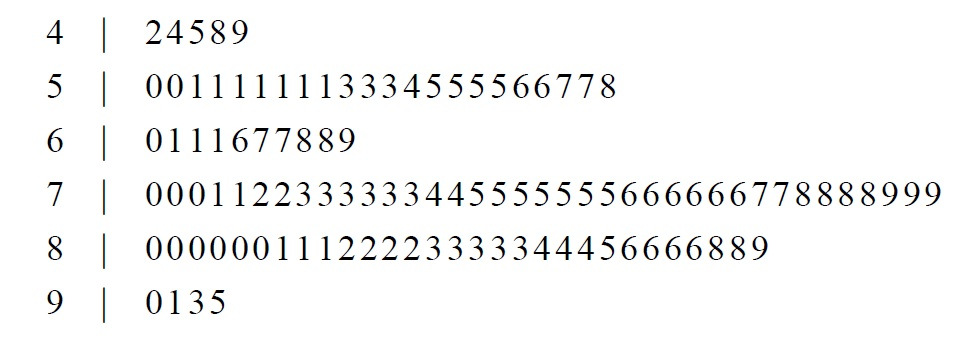
\includegraphics[scale=0.5]{stammdaten.jpg}
\end{center}

Bei diesem Beispiel sieht man, dass die Werte im Intervall [70,80) am häufigsten vorkommen.\\
Würde es sich um dreistellige Zahlen handeln, würde man die vorderste wieder als Stamm verwenden und die weiteren Stellen auf eine Stell  runden.\\(Bsp: 867 $->$ 8 = Stamm, 67 = 70 $->$ $8|7$)\\
\marginnote{  How To}

\begin{center}
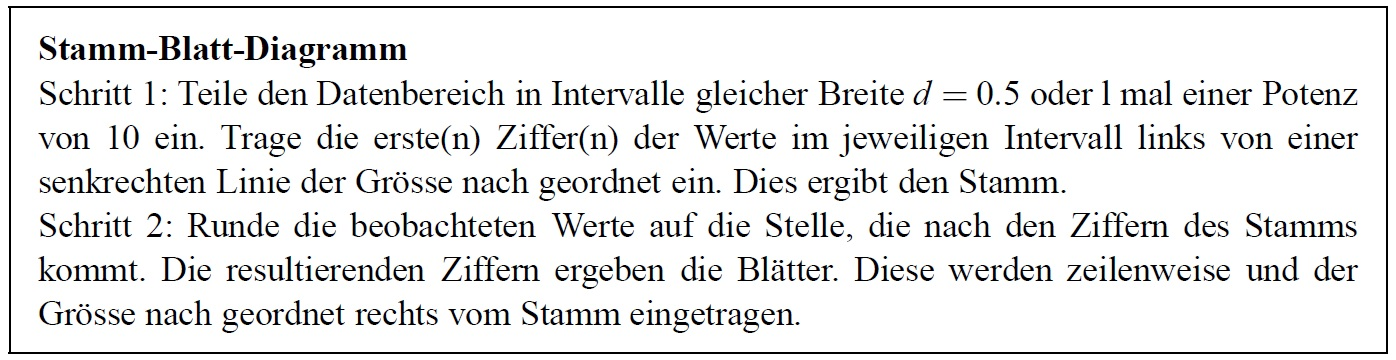
\includegraphics[scale=0.5]{beschStammBlatt.jpg}
\end{center}

\pagebreak

\subsubsection{Histogramm}
\textbf{Definition:}
\begin{itemize}
\item \textbf{Ausprägung}: Zahlenwerten, nach denen in einer "Urliste" gesucht wird. (Bsp: Summe zweier Würfel, Ausprägungen: $a_1 = 2, a_2 = 3$ \dots)
\item Die \textbf{absolute Häufigkeit} $h(a_j)$ der Ausprägung $a_j$ ist die Anzahl der $x_i \in X$ mit $x_i = a_j$.
\item Die \textbf{relative Häufigkeit} $f(a_j)$ der Ausprägung $a_j$ ist $f(a_j) = \frac{h(a_j)}{n}$.
\end{itemize}

Die Werte eines Versuchs werden in einer sogenannten Häufigkeitstabelle festgehalten:
\begin{center}
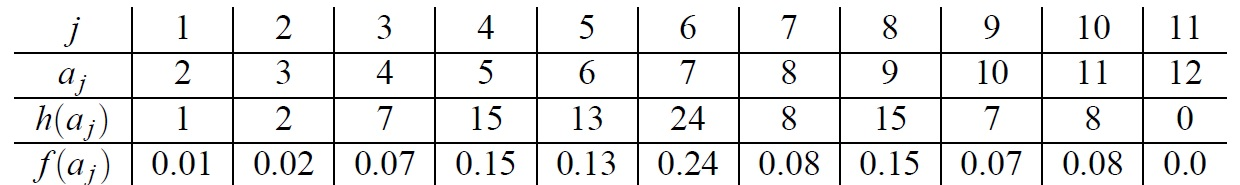
\includegraphics[scale=0.5]{haeufig.jpg}
\end{center}
Diese Werte kann man dann in einem \textbf{Histogramm} darstellen:
\begin{center}
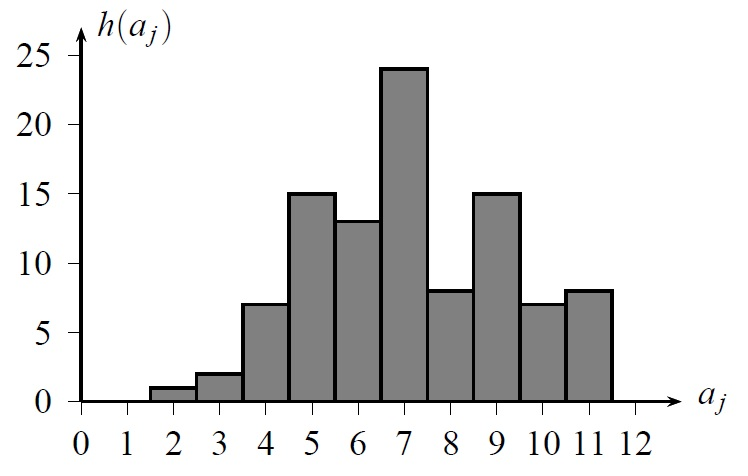
\includegraphics[scale=0.5]{histogramm.jpg}
\end{center}
In diesem Fall ist die Ausprägung diskret, somit haben wir keine Probleme dies darzustellen. Würde die Ausprägung stetig sein, so müsste man Klassen definieren, in welche die Werte eingeteilt werden, um dann ein Histogramm zu erstellen.
$$\textit{Anzahl Klassen} = \sqrt{n}, n = \textit{Umfang der Stichprobe}$$
\pagebreak
\subsubsection{Empirisiche Verteilungsfunktion}
Sei $X$ eine geordnete Stichprobe vom Umfang $n$. Somit ist die Verteilfunktion: 
$$H(x) = \frac{1}{n} \sum_{u \le x, u \in X} h(u) = \sum_{u \le x, u \in X} f(u)$$
Beispiel:
\begin{center}
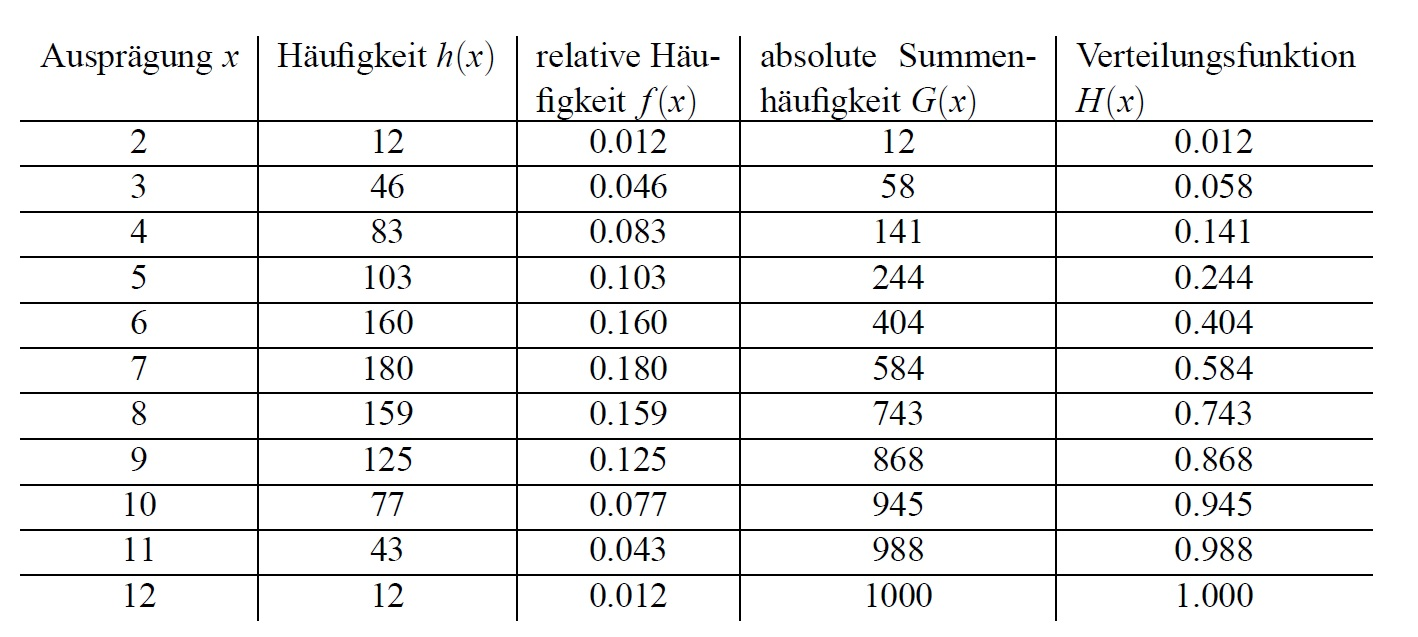
\includegraphics[scale=0.5]{verteilfunktion.jpg}
\end{center}

\subsubsection{Arbeiten mit Quantilen}
Quantile sind eine Unterteilung (vier Teile). Sie lassen sich an der Verteilfunktion leicht ablesen.\\
\begin{itemize}
\item erste Quartil: $x_{25}$
\item dritte Quartil: $x_{75}$
\item Median (zweite Quartil): $x_{50}$
\end{itemize}
\marginnote{Erklärung nächste Seite}
\begin{center}
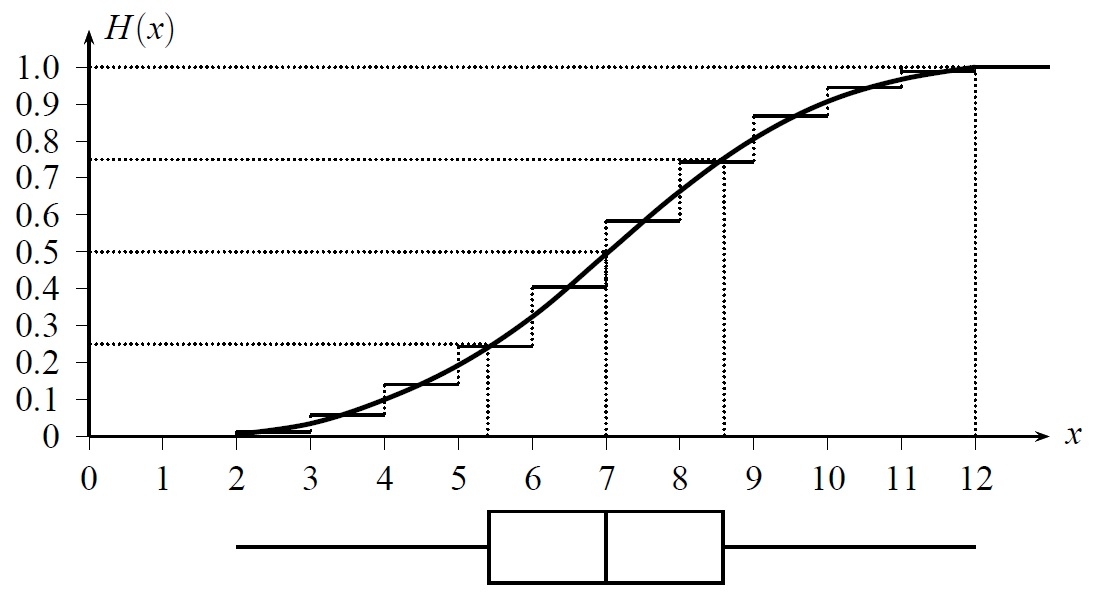
\includegraphics[scale=0.5]{quartile.jpg}
\end{center}

Bei dieser Kurve bestimmt sich das erste Quartil aus $H(x) = 0.25$, was in diesem Fall ca. 5.3 darstellt. Die anderen zwei Quartile definiert man auf die selbe Weise mit 0.5 respektive 0.75. Somit erhählt man folgende Werte:
$$x_{0.25} = 5.3, x_{0.5} = 7, x_{0.75} = 8.6$$
Der Wert $x_{0.25} = 5.3$ bedeutet, dass alle Werte die kleiner sind als 5.3 einen Stichprobenanteil von $25\%$ ausmachen.

\subsection{Statistische Masszahlen}
\subsubsection{Arithmetische Mittel}

Das \textbf{arithmetische Mittel} ist das bekannteste Lagemass. Man erhält es, indem man beobachteten Werte aufsummiert und sie durch die Anzahl der Beobachtungen dividiert.
$$\overline{x} = \frac{1}{n} \sum_{n=1}^n x_i$$
oder mit relativen Häufigkeiten:
$$\overline{x} = \sum_{i=1}^k a_if(a_i)$$
Beispiele:
\begin{center}
\fbox{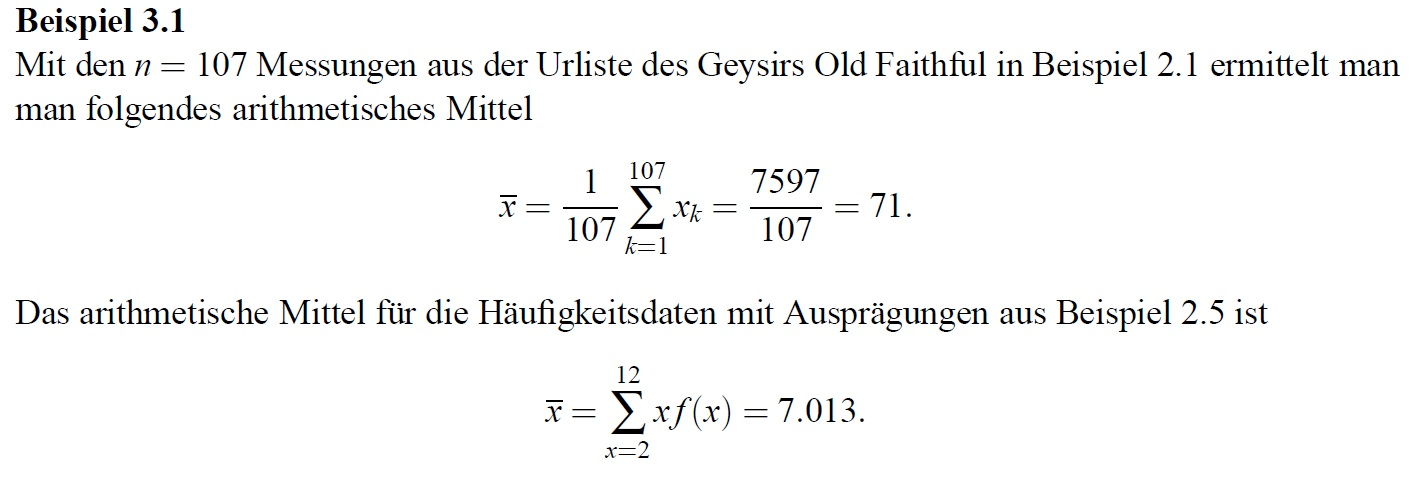
\includegraphics[scale=0.4]{beispieleAritMittel.jpg}}
\end{center}

\subsubsection{Modalwert (Modus)}
\marginnote{Definition aus Skript}
Der \textbf{Modalwert} gibt an, welche Ausprägung am häufigsten vorkommt.

\begin{center}
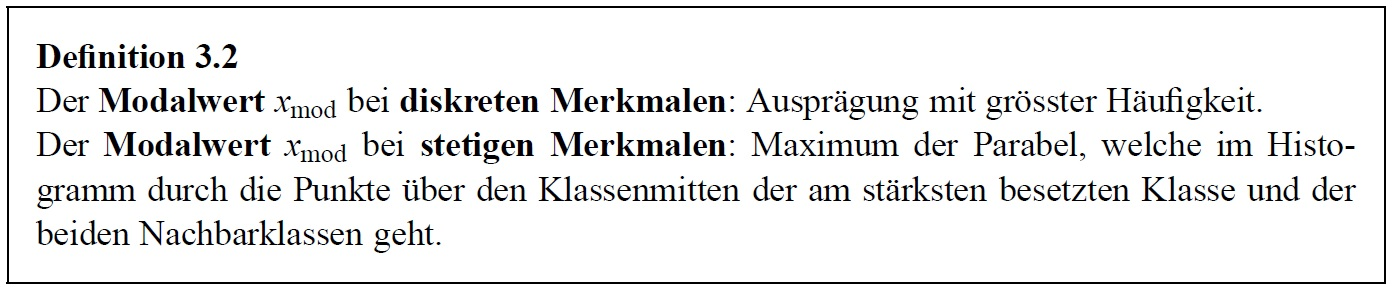
\includegraphics[scale=0.5]{defModalwert.jpg}
\end{center}

Der höchste Wert ist jeweils beim Median. Dieser wird wie folgt berechnet:
\begin{center}
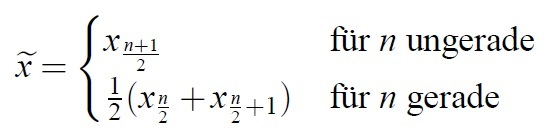
\includegraphics[scale=0.5]{medianBerech.jpg}
\end{center}

\subsubsection{Quartile}
Zur erklärung der Berechnung von Quartilen, ein Beispiel:\\
Wir wollen die Quartile für folgende Zahlen herausfinden: $0.5, 3, 4, 5, 6, 7$. Mit $n=6$ wir erhalten folgende Ergebnisse:
$$Q_1:[\frac{n+3}{4}] = [\frac{9}{4}] = [2.25],\tab Q_3:[\frac{3n+1}{4}] = [\frac{19}{4}] = [4.75]$$
Für $Q_1$ ist somit $n_1 = 2$ und $n_2 = 3$ (nächst grössere/kleinere Ganzzahl von 2.25):
$$Q_1 = (x_{n_2} - x_{n_1})\cdot \frac{n+3}{4} + x_{n_1} \cdot n_2 - x_{n_2} \cdot n_1$$
$$Q_1 = (x_3 - x_2) \cdot \frac{9}{4} + x_2 \cdot 3 - x_3 \cdot 2 = (4-3) \cdot \frac{9}{4} + 3 \cdot 3 - 4 \cdot 2 = 3.25$$
Für $Q_3$ ist $n_1 = 4$ und $n_2 = 5$:
$$Q_3 = (x_{n_2} - x_{n_1})\cdot \frac{3n+1}{4} + x_{n_1} \cdot n_2 - x_{n_2} \cdot n_1$$
$$Q_1 = (x_5 - x_4) \cdot \frac{19}{4} + x_4 \cdot 5 - x_5 \cdot 4 = (6-5) \cdot \frac{19}{4} + 5 \cdot 5 - 6 \cdot 4 = 5.75$$

\subsubsection{Standardabweichung, Varianz}
\marginnote{Definitionen aus Skript}


\begin{center}
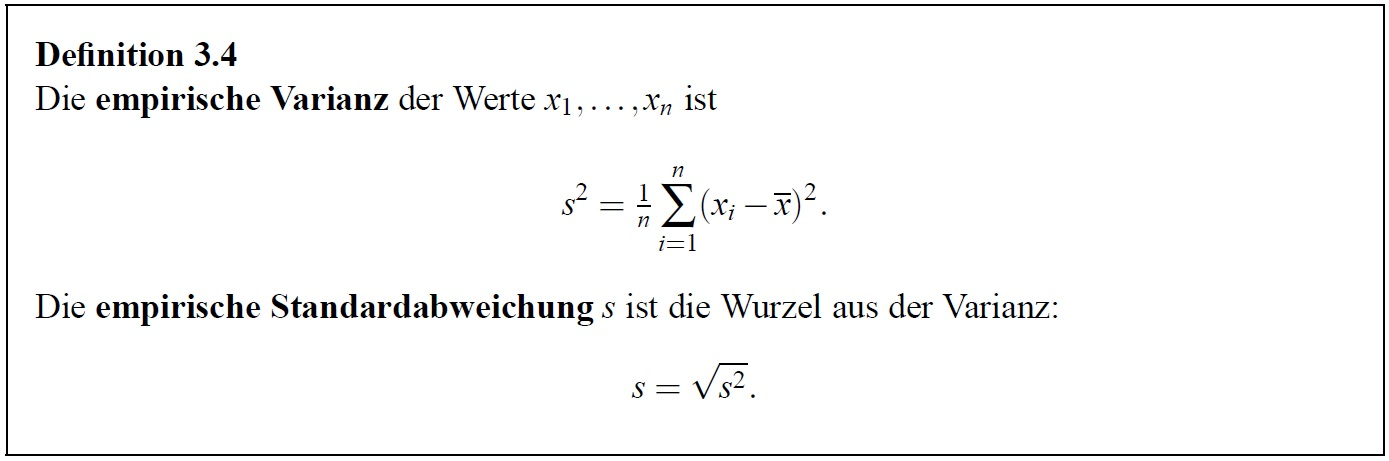
\includegraphics[scale=0.5]{defVarianz.jpg}
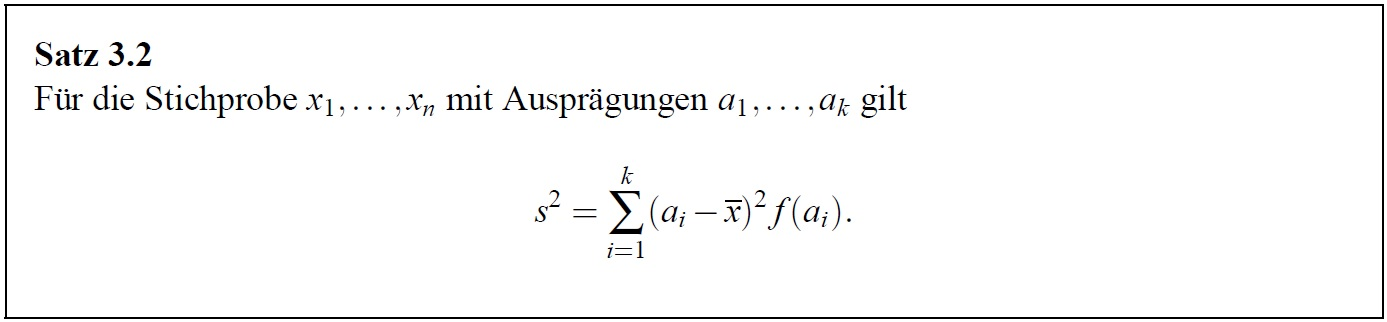
\includegraphics[scale=0.5]{defVarianz2.jpg}
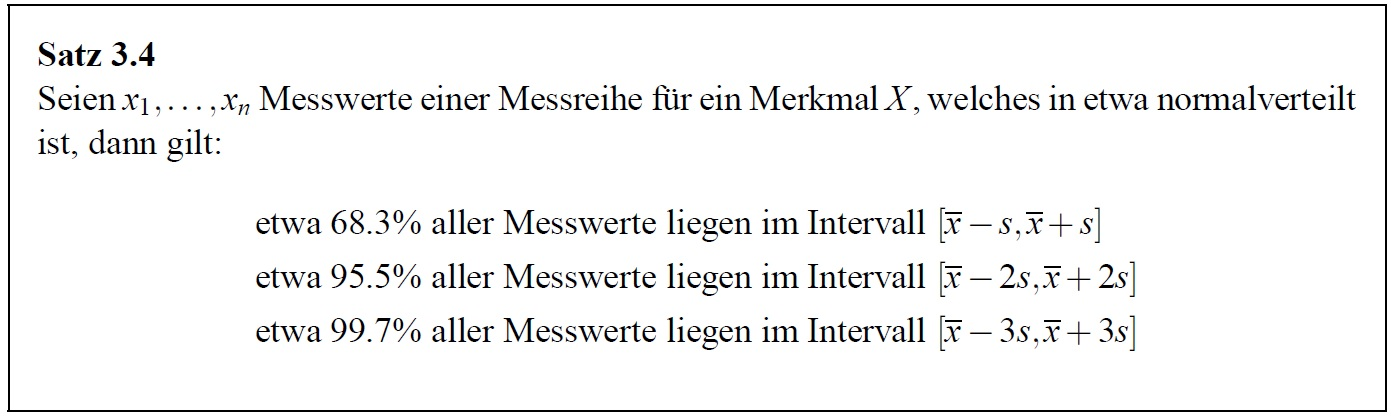
\includegraphics[scale=0.5]{bedStandardabweichung.jpg}
\end{center}


\marginnote{Beispiel aus Skript}


\begin{center}
\fbox{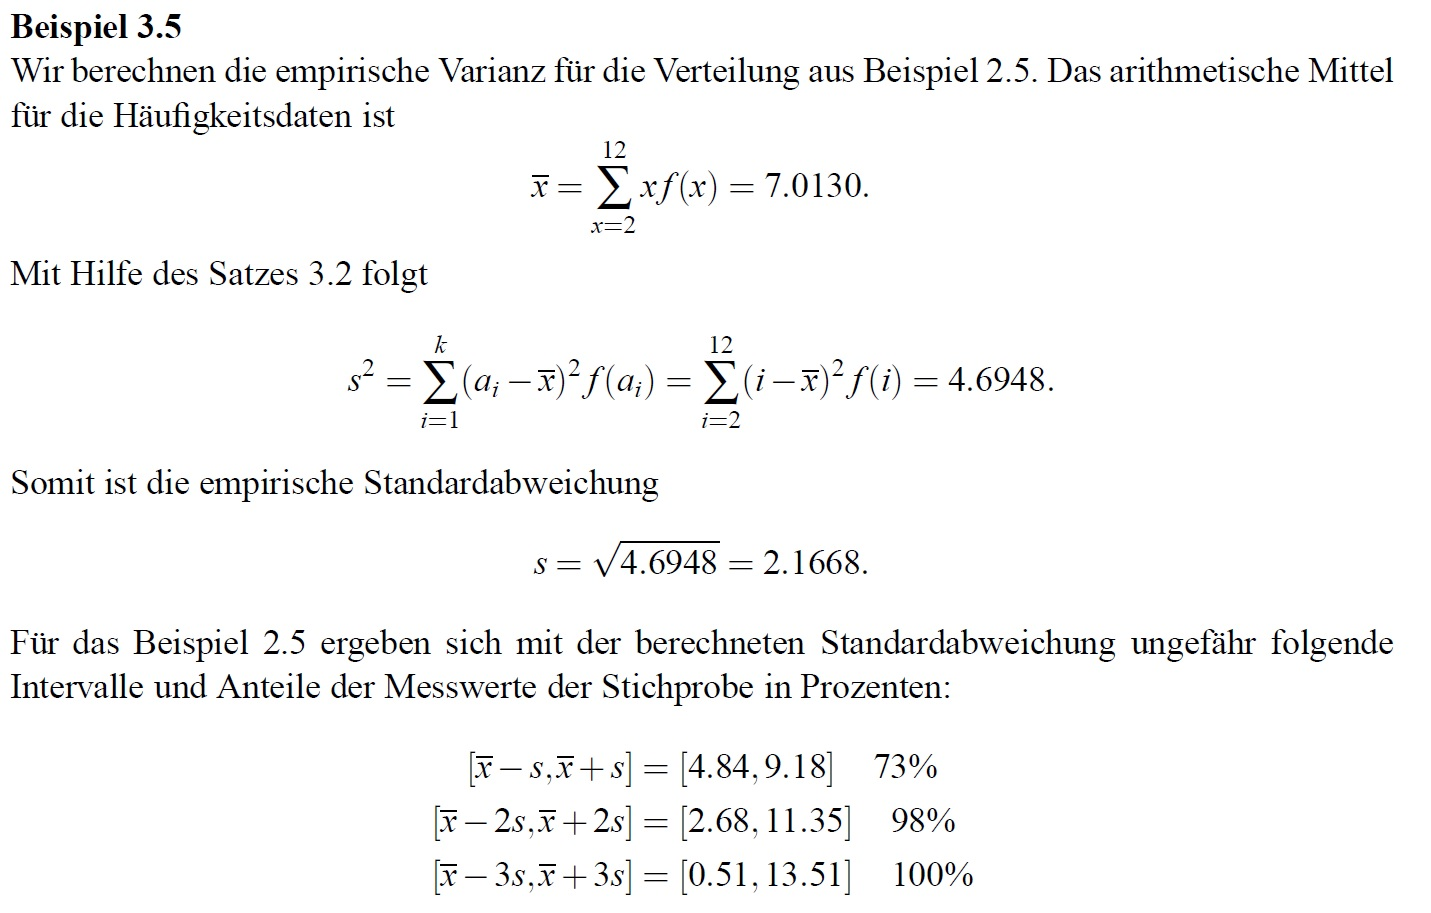
\includegraphics[scale=0.4]{bspVarianz.jpg}}
\end{center}

\subsection{Dichtekurven und Normalverteilung}

\subsubsection{Dichtekurven}
Bei den Dichtekurven geht es darum, die Histogramme durch eine glatte, stetige Funktion zu ersetzen, damit zu jedem Zeitpunkt ein genaues Resultat hat.

\begin{center}
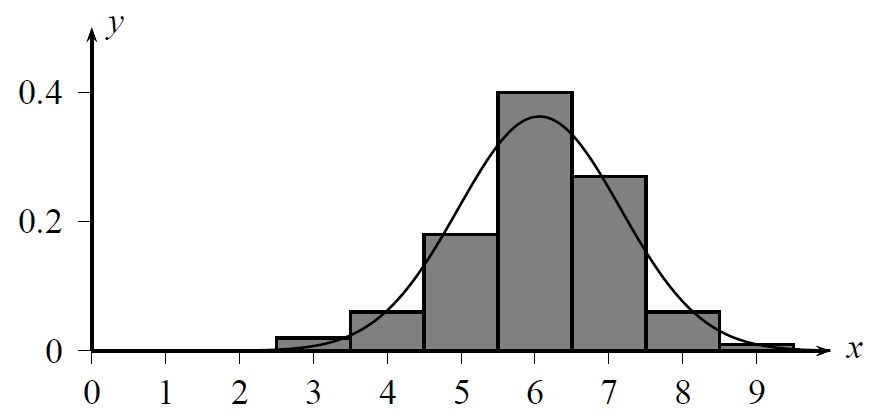
\includegraphics[scale=0.5]{histoZuStetig.jpg}
\end{center}

Die \textbf{Dichtekurve} oder kurz Dichte wird wie folgt definiert:
$$f(x)\ge 0,\tab \int_{-\infty}^\infty f(x)dx = 1$$

\subsubsection{Normalverteilung}
Normalverteilungen sind eine Art der Dichtekurven. Sie besitzen folgende Eigenschaften:
\begin{itemize}
\item symmetrisch
\item glockenförmig
\item besitzen ein Maximum
\end{itemize}
Normalverteilungen sind durch eine spezielle Formel für die Dichtekurven definiert:
\begin{eqnarray*}
f(x) &=& \frac{1}{\sigma \sqrt{2\pi}}e^{-\frac{(x-\mu)^2}{2\sigma ^2}}\\\\
x &\in & \mathbb{R}\\
\mu &\in & \mathbb{R}\\
\sigma &>& 0\\
\mu &:& Mittelwert\\
\sigma &:& Standardabweichung
\end{eqnarray*}

\begin{center}
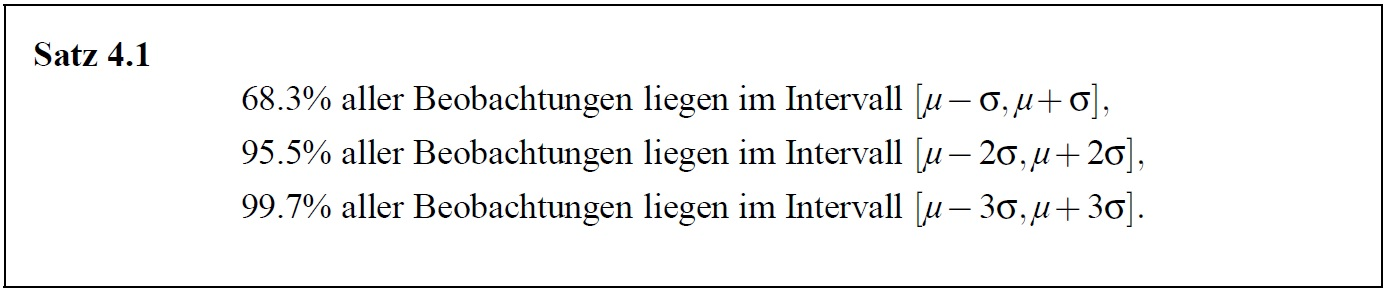
\includegraphics[scale=0.5]{bedNormalverteilung.jpg}
\end{center}


\subsection{Mehrdimensionale Verteilung}
Wir verwenden Punktewolken um zweidimensionale Elemente darzustellen. Bsp. Ein Ei mit länge und breite: x: länge / y: breite = P(x/y). Stellt man alle Punkte dar, erhält man eine Punktewolke:
\begin{center}
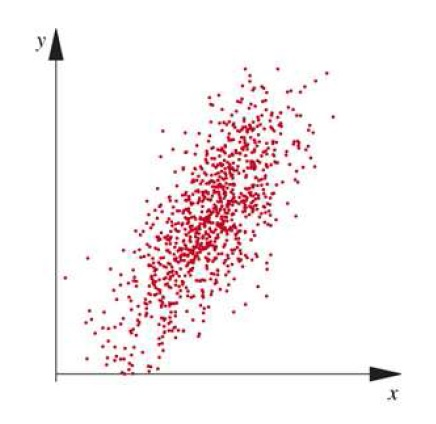
\includegraphics[scale=0.8]{punktewolke.jpg}
\end{center}

Jede Punktwolke hat eine Richtung (Beispiel oben:  Von unten links nach oben rechts). Diese Richtung nennt man \textbf{empirische Kovarianz} und wird wie folgt berechnet:
$$cov(x,y) = \frac{1}{n} \sum_{i=1}^n (x_i-\overline{x})(y_i-\overline{y})$$
Das Vorzeichen dieser Berechnung sagt aus, ob die Punktewolke eher steigt (+) oder fällt (-).
\pagebreak

\marginnote{Nur die Formel ohne Erklärung}
Definition des \textbf{empirischen Korrelationskoeffizienten}:
$$r(x,y) = \frac{1}{n} \sum_{i=1}^n \frac{(x_i-\overline{x})}{s(x)}\cdot \frac{(y_i-\overline{y}}{s(y)}$$

\pagebreak

\section{Wahrscheinlichkeitsrechnung}

\subsection{Begriffe der Wahrscheinlichkeit}
Benennung der Begriffe mit Beispiel
\begin{itemize}
\item Zufallsgerät: Münze
\item Zufallsexperiment: Münze werfen
\item Ergebnis: Kopf oder Zahl (jeweils alle möglichen Ergebnisse)
\item Ergebnisraum: Münze wird 3 mal geworfen: alle möglichen Ergebnisse nach diesem Versuch. (Zahl / Kopf / Kopf, Kopf / Zahl / Kopf,...)
\item Ereignis: Wieviel mal wurde Kopf geworfen.
\end{itemize}
Rechenregeln für Mengen: 
\begin{center}
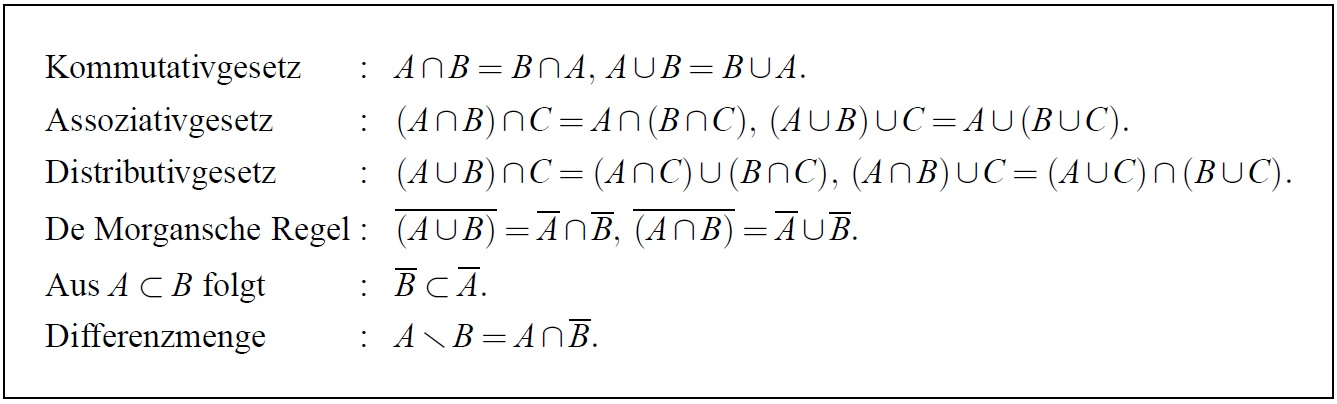
\includegraphics[scale=0.5]{rechenregeln.jpg}
\end{center}
Verknüpfungen von Ereignissen:
\begin{center}
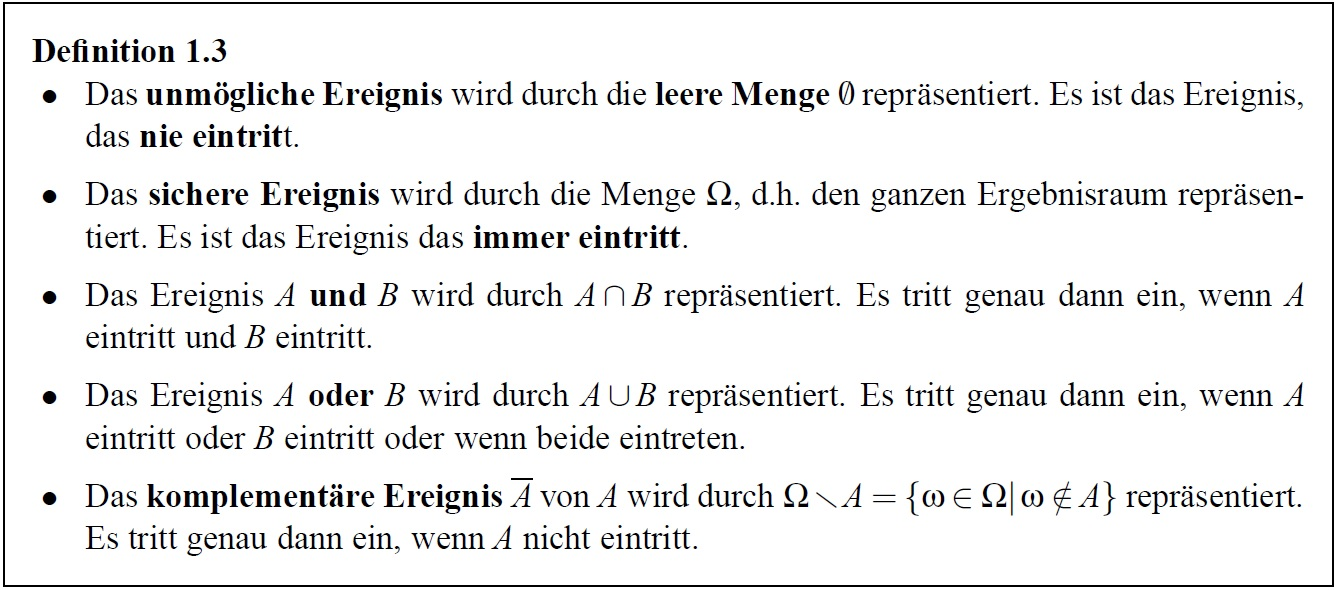
\includegraphics[scale=0.5]{verkEreignisse.jpg}
\end{center}
\pagebreak
\subsection{Wahrscheinlichkeitsauffassungen}

\subsubsection{Klassische Wahrscheinlichkeit}

Bei der klassischen Wahrscheinlichkeit (auch Laplace-Wahrscheinlichkeit) geht man davon aus, dass alle Ergebnisse eines Zufallsexperimentes die gleiche Wahrscheinlichkeit haben. (Bsp. Kopf oder Zahl). Folgende Formel wird verwendet für die Berechnung:
$$P(A) = \frac{|A|}{n} = \frac{\textit{Anzahl der Elemente von A}}{\textit{Anzahl der Elemente von }\Omega}$$

\subsubsection{Geometrische Wahrscheinlichkeit}

Analog zur Klassischen Wahrscheinlichkeit gibt es eine Gemoetrische Wahrscheinlichkeit. Diese wird im Raum $\mathbb{R}^n$ angewendet. Folgende Formeln gelten falls $A \subseteq \mathbb{R}^n$:

\marginnote {Aus dem Skript kopiert}

\begin{center}
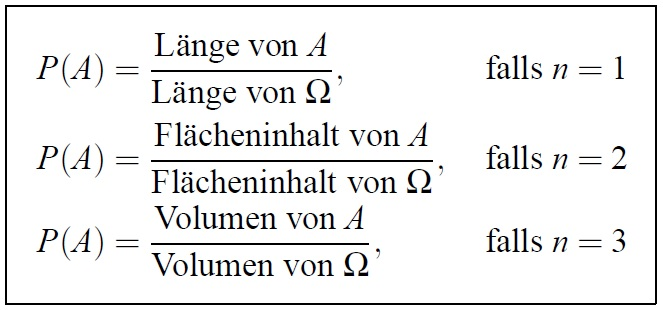
\includegraphics[scale=0.7]{geoWahrscheinlichkeit.jpg}
\end{center}

\marginnote{Beispiel}
Es werden zwei Zufallszahlen generiert. Wir interessieren uns für alle Zahlenpaare $(x,y) \in \mathbb{R}^2$, die höchstens 0.5 voneinander abeweichen.\\
Wir haben: $$\Omega = \{(x,y) \in \mathbb{R}^2 | 0 \le x \le 7, 0 \le y	 \le 7\}$$
Somit lässt sich das Ereignis A wie folgt formulieren:
$$A = \{(x,y) \in \Omega || x-y | \le 0.5\}$$
Die Wahrscheinlichkeit, dass sich die zwei Zahlen um höchstens 0.5 unterscheiden ist somit:
$$P(A) = \frac{\textit{Flächeninhalt von A}}{\textit{Flächeninhalt von }\Omega} = \frac{7^2 - 6.5^2}{7^2} = 0.138$$

\pagebreak
\subsubsection{Statische Wahrscheinlichkeit}

Ist nach $n$ Versuchswiederholungen $n_A$-mal das Ereignis $A$ eingetreten, so ist
$$h_n(A) = \frac{n_A}{n}$$
die relative Häufigkeit von $A$. Die \textbf{statische Wahrscheinlichkeit} von $A$ ist dann ein Grenzwert:
$$P(A) = \lim_{n->\infty} h_n(A)$$
\marginnote{Beispiel}
\\Eine faire Münze wurde 50mal geworfen. 32 mal erschien Zahl und 18 mal Kopf. Aufgrund dieser Statistik ist die relative Häufigkeit von $A = \{Zahl\}$:
$$h_{50} = \frac{32}{50}=0.62$$
Dies wird nun fortgeführt und mit 10000 Versuchen:
$$h_{10000} = \frac{4948}{10000} = 0.4948$$
Die relative Häufigkeit scheint sich bei grossem $n$ also einzupegeln, wir vermuten somit:
$$P(A) = \lim_{n->\infty} h_n(A) = 0.5$$

\subsection{Aximoatische Wahrscheinlichkeit}

\subsubsection{Diskreter endlicher Stichprobenraum}

\marginnote{Beispiel}
Ein Spielautomat gibt bei Betätigung einer der nebenstehenden Zahlen aus:\\$1,2,3,4,5$ und zwar mit folgenden Wahrscheinlichkeiten:
\begin{center}
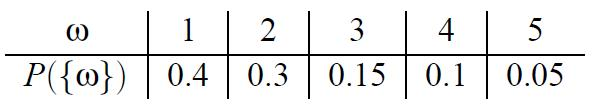
\includegraphics[scale=0.5]{wahrscheinlichkeiten35.jpg}
\end{center}
Ereignis $(A)$: es erscheint eine ungerade Zahl, also $A=1,3,5$.\\
Wie gross ist die Wahrscheinlichkeit?\\
$$P(A) = 0.4 + 0.15 + 0.05 = 0.6$$
\\
\marginnote{Beispiel}
Ein Gefäss enthält 5 weisse und 2 schwarze Kugeln. Es werden miteinander 2 Kugeln herausgezogen. (Reihenfolge spielt keine Rolle).\\
Der Ergebnisraum ist:
$$\Omega = \{ (s,s), (s,w), (w,w) \}$$
Wie gross ist die Wahrscheinlichkeit der Elementarereignisse in $\Omega$?
\pagebreak
\begin{center}
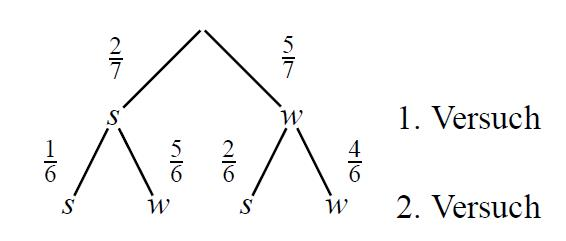
\includegraphics[scale=0.5]{baumstruktur37.jpg}
\end{center}
Diese Wahrscheinlichkeiten werden Anschliessend multipliziert und man erhält die Schlussendlichen Wahrscheinlichkeiten. (Achtung: Reihenfolge spielt keine Rolle, somit werden die Wahrscheinlichkeiten für (s,w) und (w,s) zusammengezählt)\\\\
\marginnote{Bemerkung}
Falls es sich um eine Aufgabe handelt, bei der die Anzahl versuche herausgefunden werden muss um einen Bestimmten Prozentsatz zu erreichen, ist es hilfreich die ersten 3-4 Durchgänge auszurechnen und dann eine auf $n$ bezogene Formel herauszufinden. Dann kann diese Formel mit dem Prozentsatz gleichgestellt werden und herausgefunden werden wieviele Würfe es braucht.

\subsubsection{Unendlicher diskreter Ergebnisraum}

\marginnote{Beispiel}
Eine Münze wird so oft geworfen bis Kopf zum ersten mal erscheint. Dieser Zufallsversuch hat unendlich viele Ergebnisse und der Ergenisraum	ist:
$$\Omega = \{(K), (Z,K), (Z,Z,K), \cdots \}$$
Dadurch erhalten wir folgende Wahrscheinlichkeiten:
\begin{center}
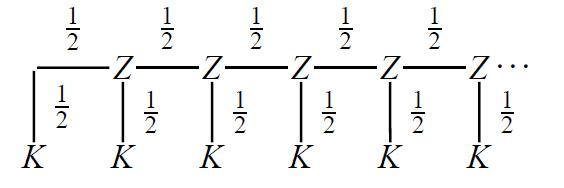
\includegraphics[scale=0.5]{muenzbaum.jpg}
\end{center}
\begin{center}
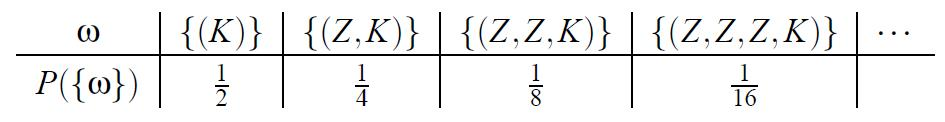
\includegraphics[scale=0.5]{muenzwahrsch.jpg}
\end{center}
Die Summe über alle Elementarereignisse aus dem Ereignisbaum muss 1 ergeben. Dies ist tatsächlich der Fall:
$$P(\Omega) = P (\{K\})+P(\{Z,K\})+\cdots = \frac{1}{2}+\frac{1}{4}+\cdots = \frac{\frac{1}{2}}{1-\frac{1}{2}} = 1$$
\marginnote{Beispielresultate aus Skript}
\begin{center}
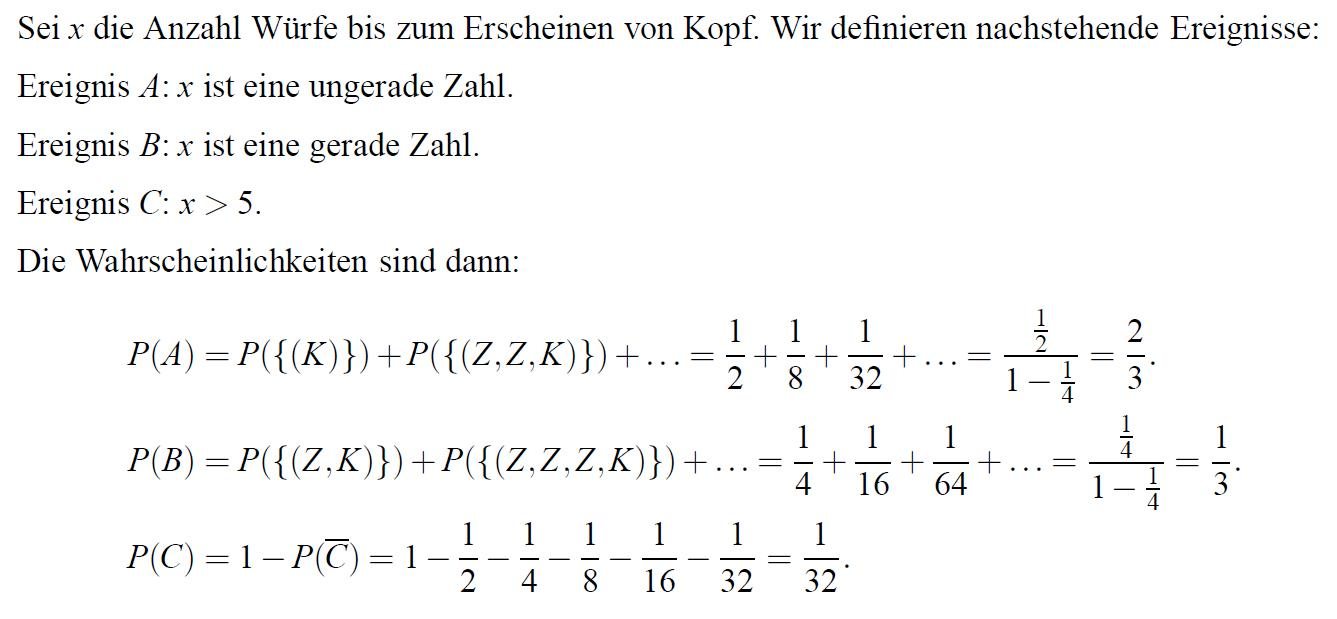
\includegraphics[scale=0.4]{muenzbsp.jpg}
\end{center}

Notiz: Bedingte Wahrscheinlichkeit
\subsection{Bedingte Wahrscheinlichkeit}
\subsubsection{Definition}
Bei der bedingten Wahrscheinlichkeit ist nicht mehr der gesamte Ergebnisraum $\Omega$ verfügbar. Für das Eintreten von Eregnis A, muss Ereignis B vorher eingetreten sein.\\Bezeichnung: $P(A|B)$\\ (Wahrscheinlichkeit von A, unter Voraussetzung, dass B eingetroffen ist.)\\\\
Berechnung:
$$P(A|B) = \frac{\textit{günstige Fälle}}{\textit{mögliche Fälle}} = \frac{|A \cap B|}{|B|}$$
Weiter gilt:
$$P(A\cap B) = \frac{|A\cap B|}{|\Omega|}, P(A) = \frac{|A|}{|\Omega|}, P(B) = \frac{|B|}{|\Omega|}$$
Damit folgt für die bedinte Wahrscheinlichkeit:
$$P(A|B) = \frac{|A\cap B|}{|B|} = \frac{\frac{|A\cap B|}{|\Omega|}}{\frac{|B|}{|\Omega|}}=\frac{P(A\cap B)}{P(B)}, P(B)>0$$
Für zwei Ergebnisse gelten folgende Gesetzte:
$$P(A\cup B) = P(A) + P(B)\textit{, falls } A\cap B = 0$$
$$P(\overline{A})= 1-P(A)$$  
Wahrscheinlichkeit des Eintretens von $A$ und $B$ berechnen:\\
\textbf{Produktsatz}:
$$P(A\cap B) = P(A|B)\cdot P(B)\textit{ oder } P(A\cup B) = P(B|A) \cdot P(A)$$

\subsubsection{Unabhängigkeit von zwei Ereignissen}
Ist die Wahrscheinlichkeit zweier Ereignisse voneinander unabhängig, so nennt man dies stochastik unabhängig.
$$P(A|B) = P(A)$$
Daraus ergibt sich folgende Formel:\\
Seien $A$ und $B$ beliebige unabhängige Ereignisse eines Zufallsversuchs. Dann gilt
$$P(A\cap B) = P(A) \cdot P(B)$$
Die Wahrscheinlichkeit das A und B eintrifft, ist das Produkt der Wahrscheinlichkeit von A und B (siehe alles weiter oben).

\subsubsection{Totale Wahrscheinlichkeit}
Auch Partition genannt:
\begin{center}
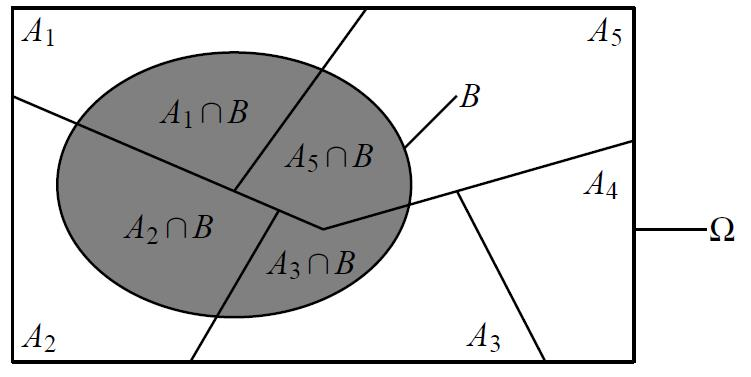
\includegraphics[scale=0.5]{partition.jpg}
\end{center}
Satz von der totalen Wahrscheinlichkeit:
$$P(B)=\sum_{k=1}^n P(B|A_k)\cdot P(A_k)$$

\subsubsection{Satz von Bayes}
Seien die Ereignisse $A_1,\cdots ,A_n$ eine Partition vom Ergebnisraum $\Omega$, und sei $B \subseteq \Omega$ ein Ereignis mit $P(B) > 0$. Dann gilt:
$$P(A_k,B) = \frac{P(B|A_k)\cdot P(A_k)}{\sum_{i=1}^n P(B|A_i)\cdot P(A_i)}, k=1,\cdots,n$$


\end{document}